\documentclass[11pt]{beamer}
\usepackage{amsfonts,amsmath,amsthm,amssymb}
\theoremstyle{plain}
\newtheorem{conjecture}{Conjecture}[section]
\usepackage{mathtools,mathptmx,listings,forest,enumitem}
\usepackage{graphicx}
\usepackage{pgfplots}
\pgfplotsset{compat=newest}
% plotting things
\usepackage{graphicx}
\graphicspath{{images/}}
\usepackage{tikz-cd}
\pgfplotsset{compat=1.15}
\usepackage[
	backend=biber,
	style=verbose,
	sorting=ynt
]{biblatex}
\addbibresource{references.bib}
\usetheme{Madrid}
\usepackage{float,mathtools,dirtytalk,ulem,csquotes,cancel,hyperref}
\author[] % (optional)
{Emon Hossain\inst{1}}

\institute[University of Dhaka] % (optional)
{
  \inst{1}%
  Lecturer\\MNS department\\Brac University
}

\date[] % (optional)
{\textsc{Lecture-01}}


\title[]{MAT215: Complex Variables And Laplace Transformations}

\setbeamertemplate{navigation symbols}{}


\AtBeginSection[]
{
  \begin{frame}
    \frametitle{Table of Contents}
    \tableofcontents[currentsection]
  \end{frame}
}

\usepackage{Kyushu}

% \usetheme{Frankfurt}

\begin{document}
\begin{frame}
\titlepage
\end{frame}

\begin{frame}{Motivation}
    The Fourier Transform tells us which frequencies or sinusoids are present in a function. On the other hand, the Laplace Transformation tells us which sinusoids and exponentials are present in a function. That means that the Fourier transform is just a slice of the Laplace transform.   
    $$
    \mathcal F(\omega)=\int_{-\infty}^\infty f(t) e^{-i\omega t}dt
    $$
    If you put in a pure cosine curve, then the Fourier gives one spike. Okay, now start with $f(t)=e^{-t}\sin t, t\geq 0$ then, 
    \begin{align*}
        \mathcal F(\omega) &= \int_{0}^\infty e^{-t}\sin t\: e^{-i\omega t}dt\\
        &= \frac{1}{1+(1+i\omega)^2}\\
        &= \frac{1}{2-\omega^2+2\omega i}
    \end{align*} 
\end{frame}

\begin{frame}{Fourier Transform (Magnitude)}
    \begin{figure}
        \centering
        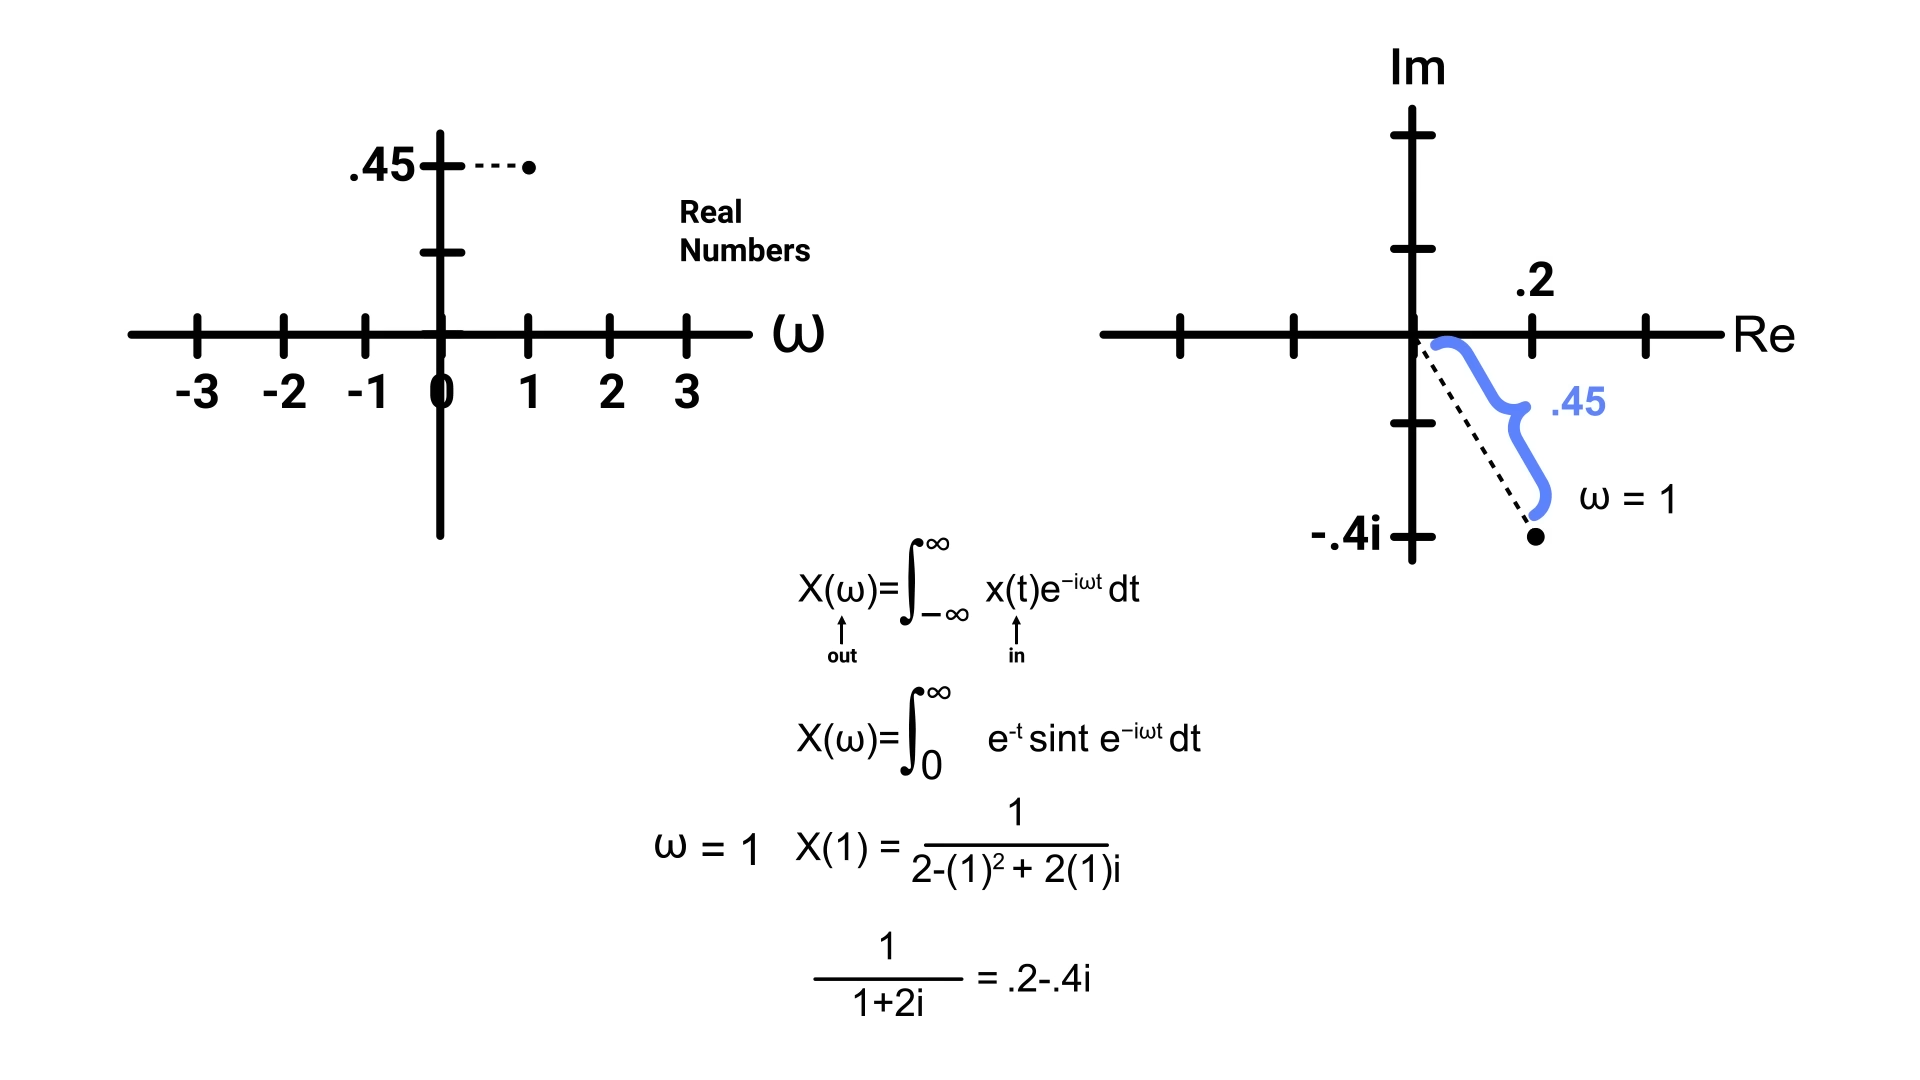
\includegraphics[width=\linewidth]{Laplace_01_graph.png}
    \end{figure}
    If we were to plot all the magnitudes for any input $\omega$, we would get the magnitude of the Fourier Transform.
\end{frame}

\begin{frame}{Visual Fourier}
    \begin{figure}
        \centering
        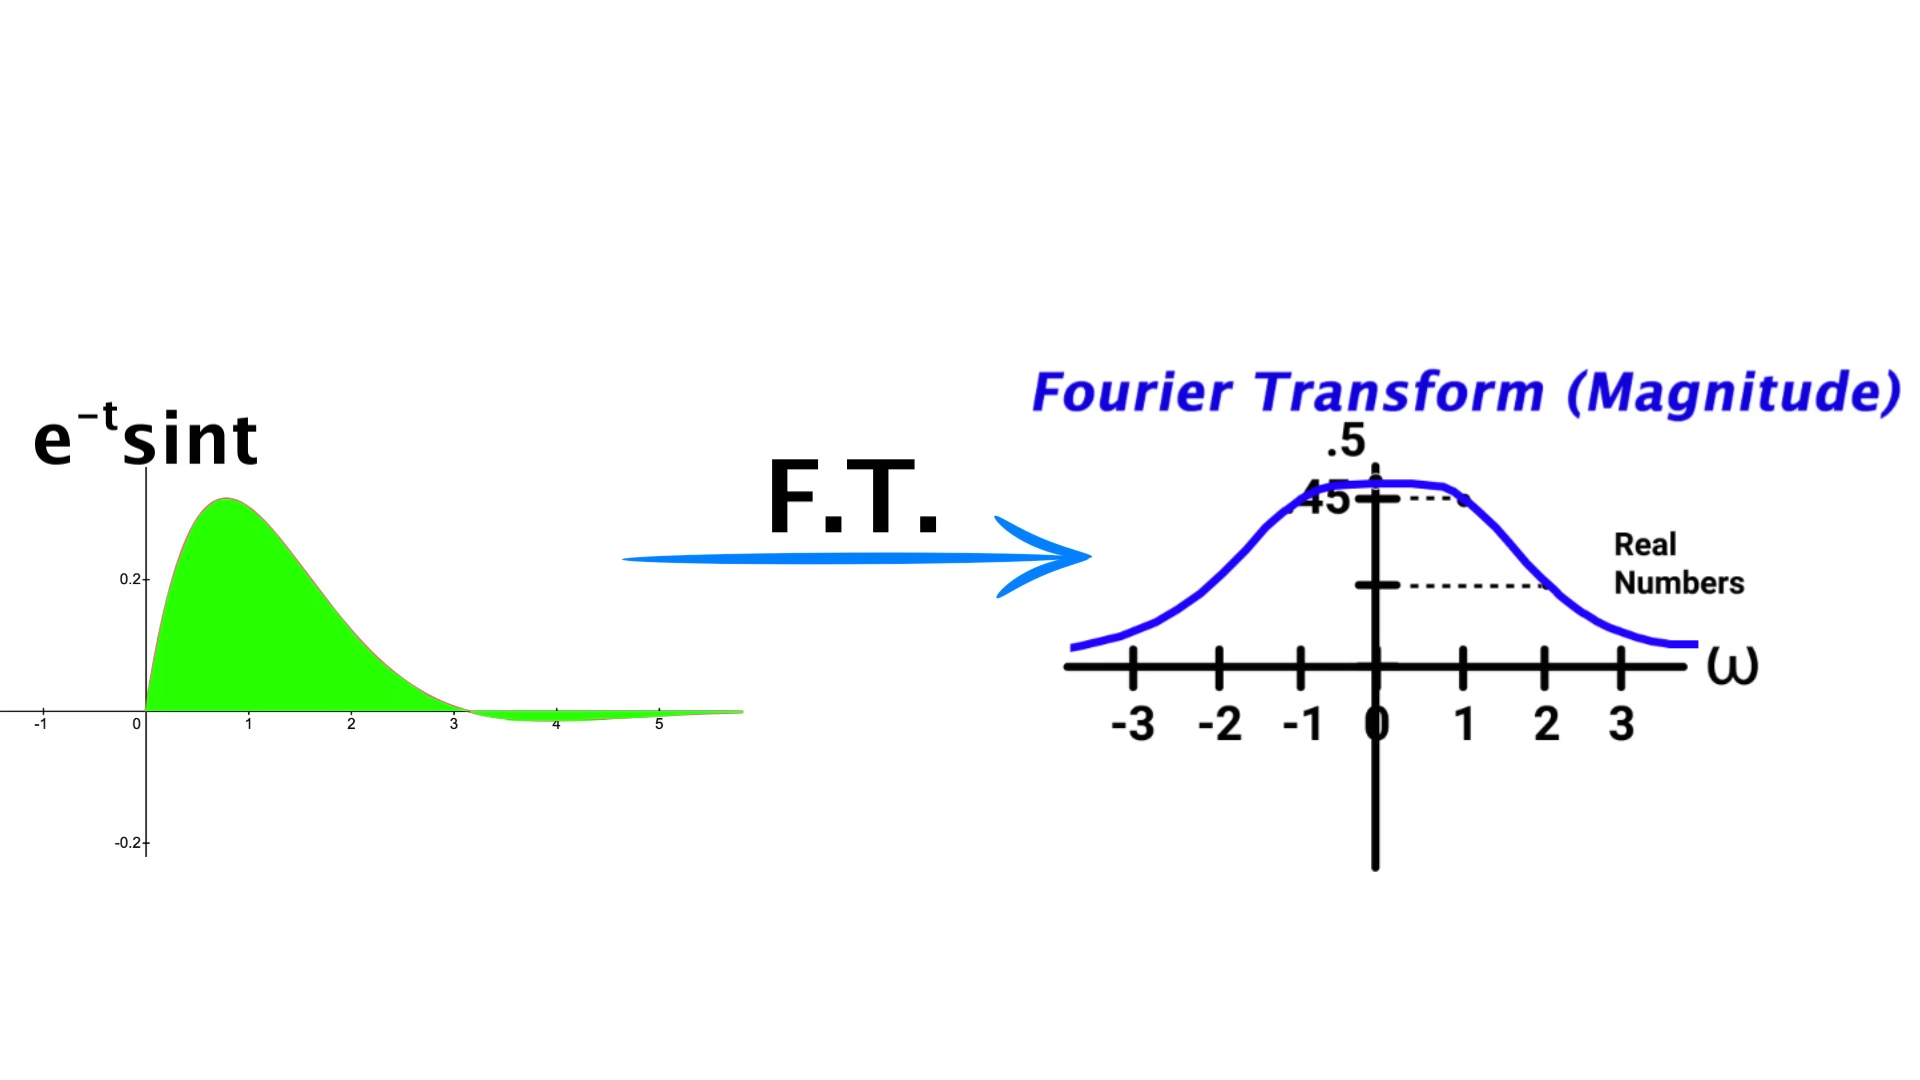
\includegraphics[width=1\linewidth]{Fourier_01_graph.png}
    \end{figure}
\end{frame}


\begin{frame}{Laplace Transform}
    Where the Laplace Transform is,
    \begin{align*}
        \mathcal L(s) &= \int_0^\infty f(t) e^{-st}dt, s\in\mathbb C\\
        &\stackrel{s=\alpha+i\omega}{=} \int_0^\infty f(t) e^{-(\alpha+i\omega)t}dt\\
        &= \int_0^\infty f(t) e^{-\alpha t}e^{-i\omega t}dt
    \end{align*}
    That means the Laplace Transform of $f(t)$ is the Fourier transform of $f(t)e^{-\alpha t}$. Do the same computation for $f(t)=e^{-t}\sin t,t\geq 0$. Then,
    \begin{align*}
        \mathcal L(s) &= \frac{1}{1+(1+s)^2}\\
        &= \frac{1}{1+(1+\alpha+i\omega)^2}
    \end{align*}
If $\alpha=0$, we get the exact Fourier Transform. 
\end{frame}

\begin{frame}{Laplace Transform}
    \begin{figure}
        \centering
        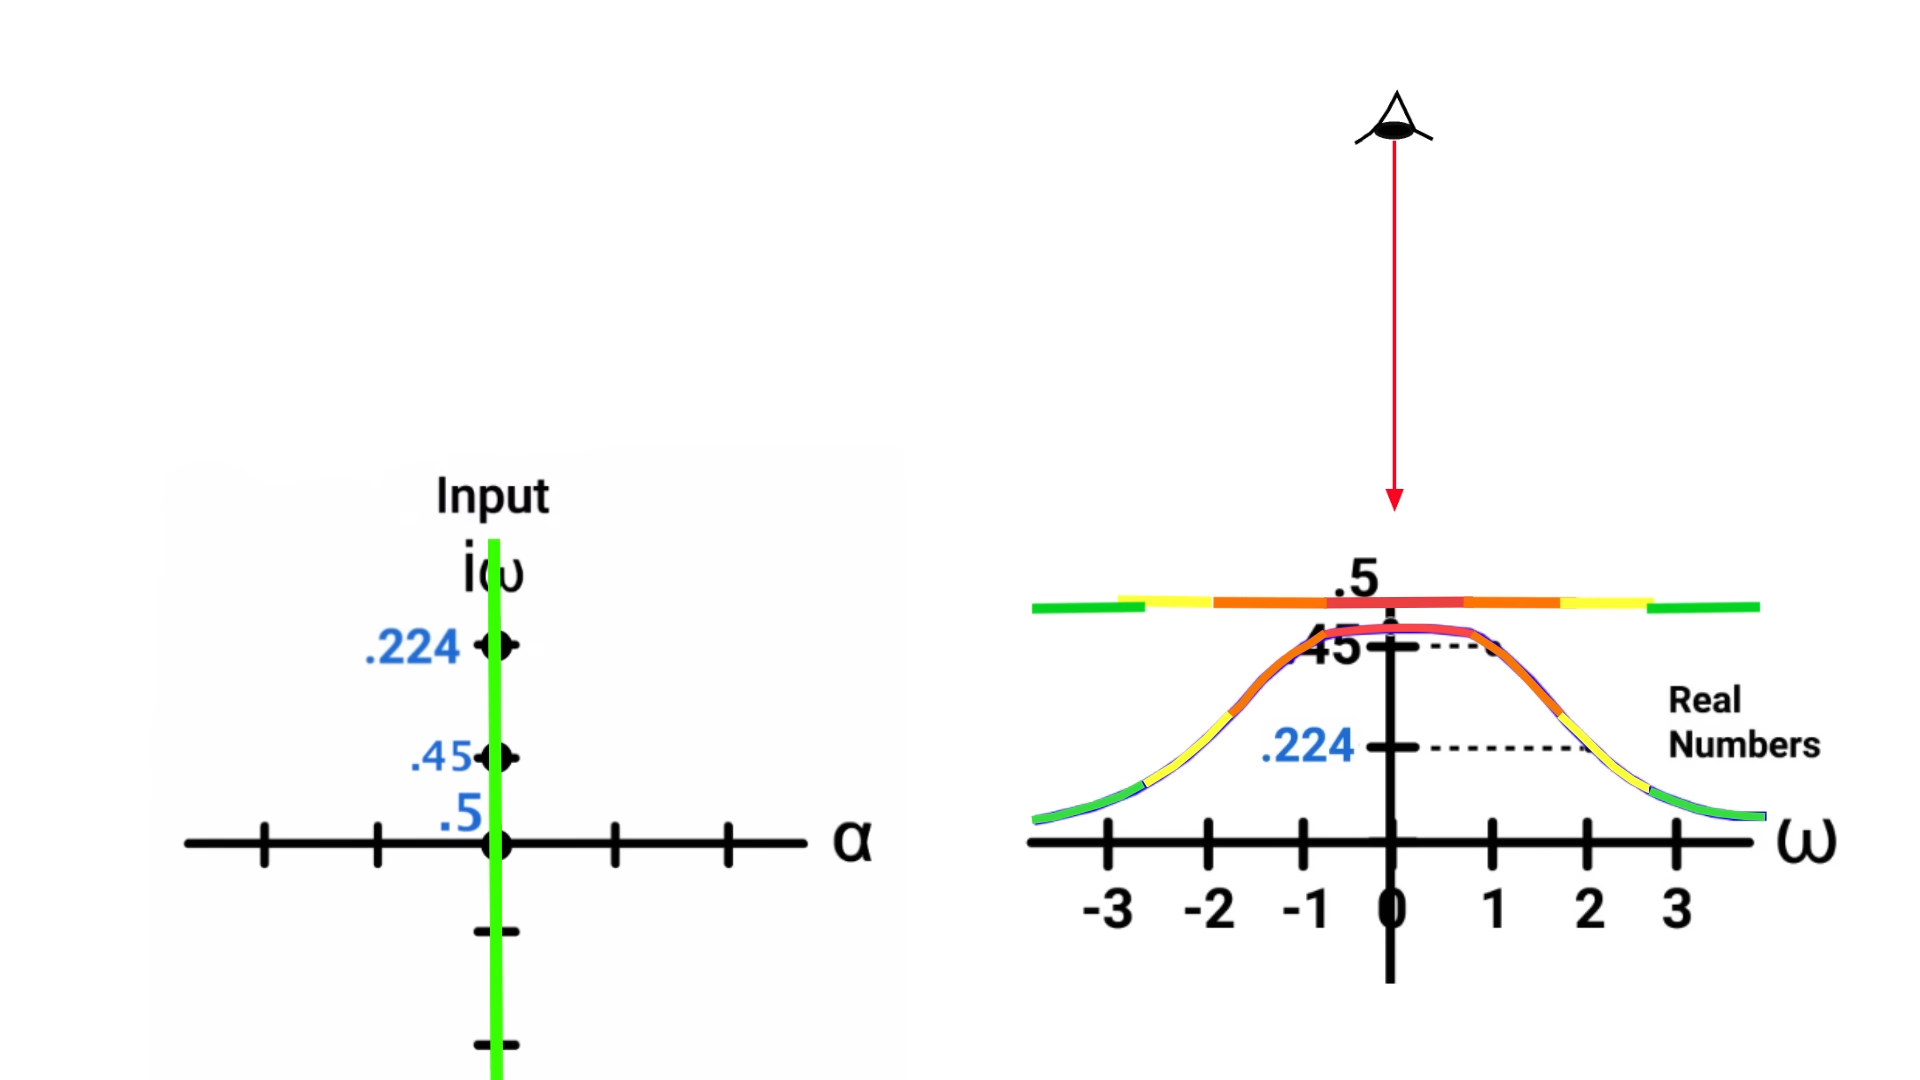
\includegraphics[width=1\linewidth]{Laplace_02_graph.png}
    \end{figure}
\end{frame}

\begin{frame}{Laplace Transform}
    \begin{figure}
        \centering
        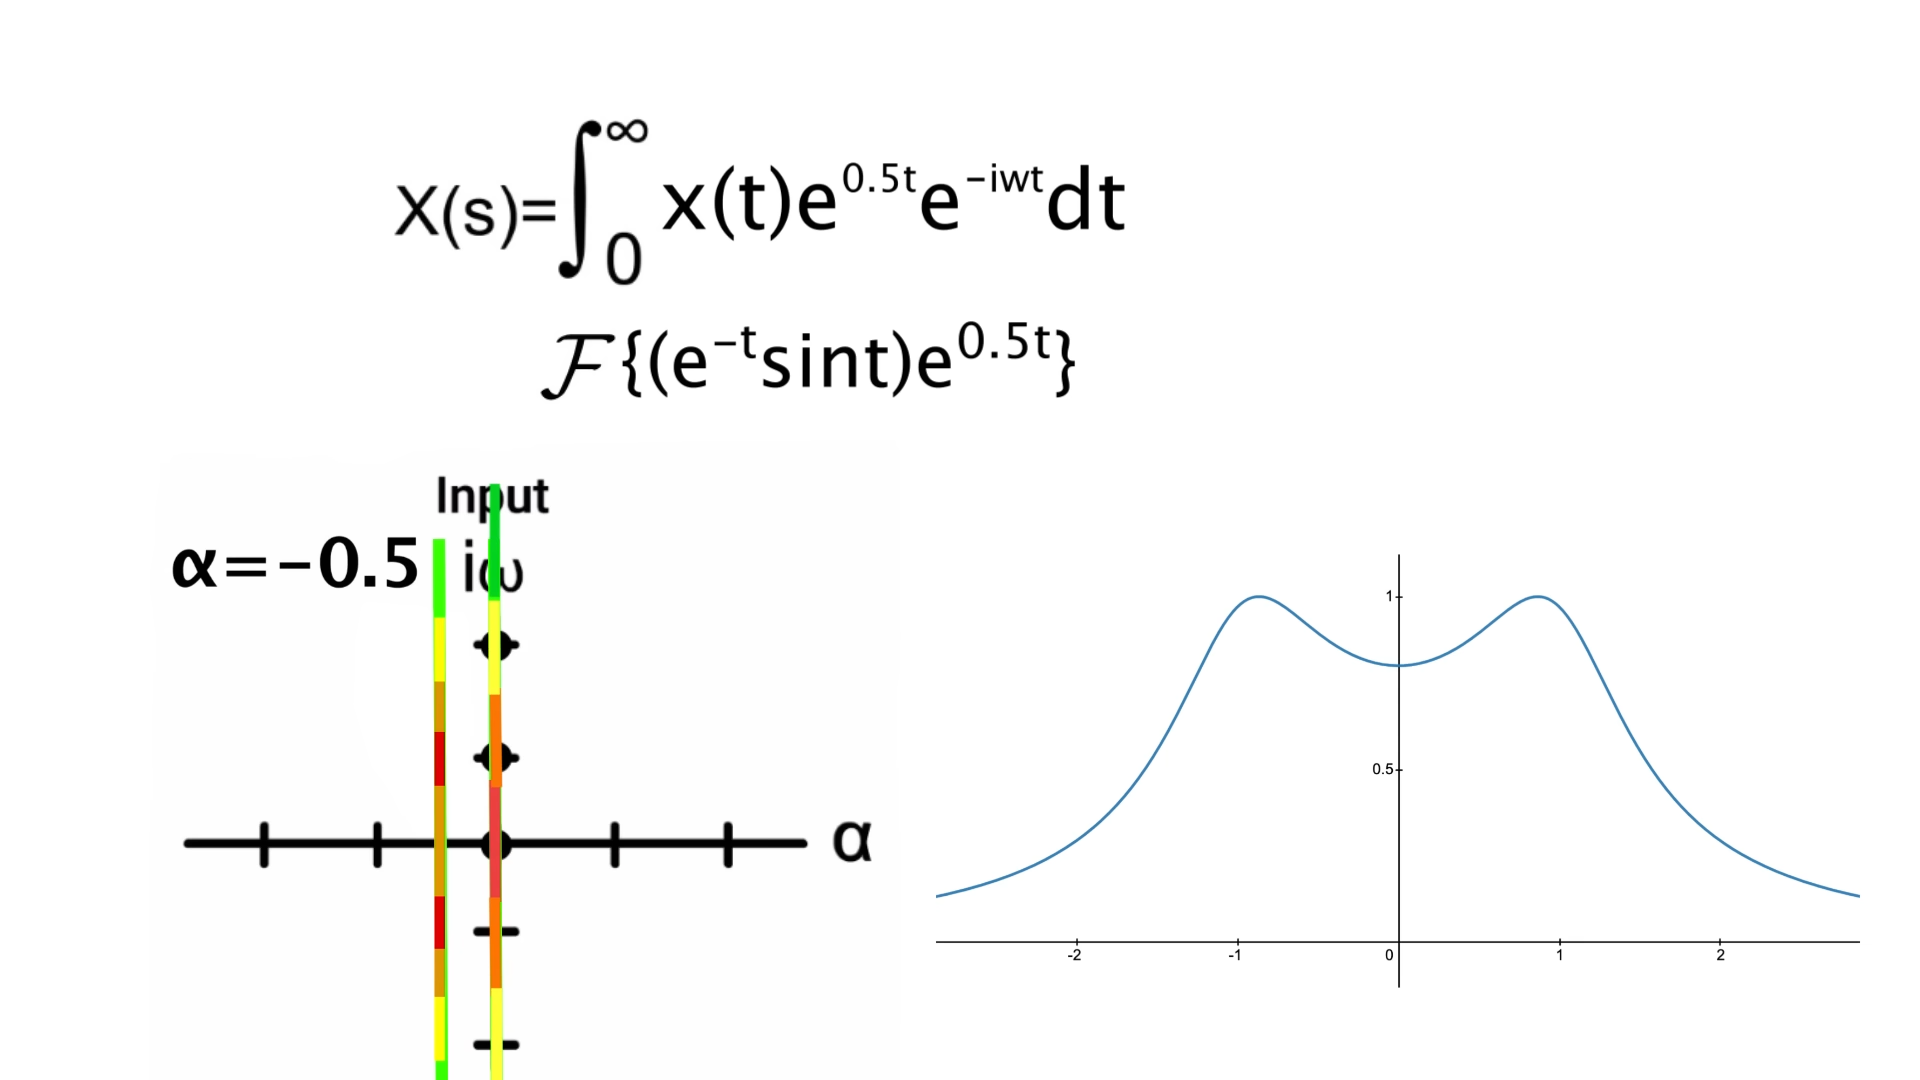
\includegraphics[width=1\linewidth]{Laplace_022_graph.png}
    \end{figure}  
\end{frame}

\begin{frame}{Laplace Transform}
    \begin{figure}
        \centering
        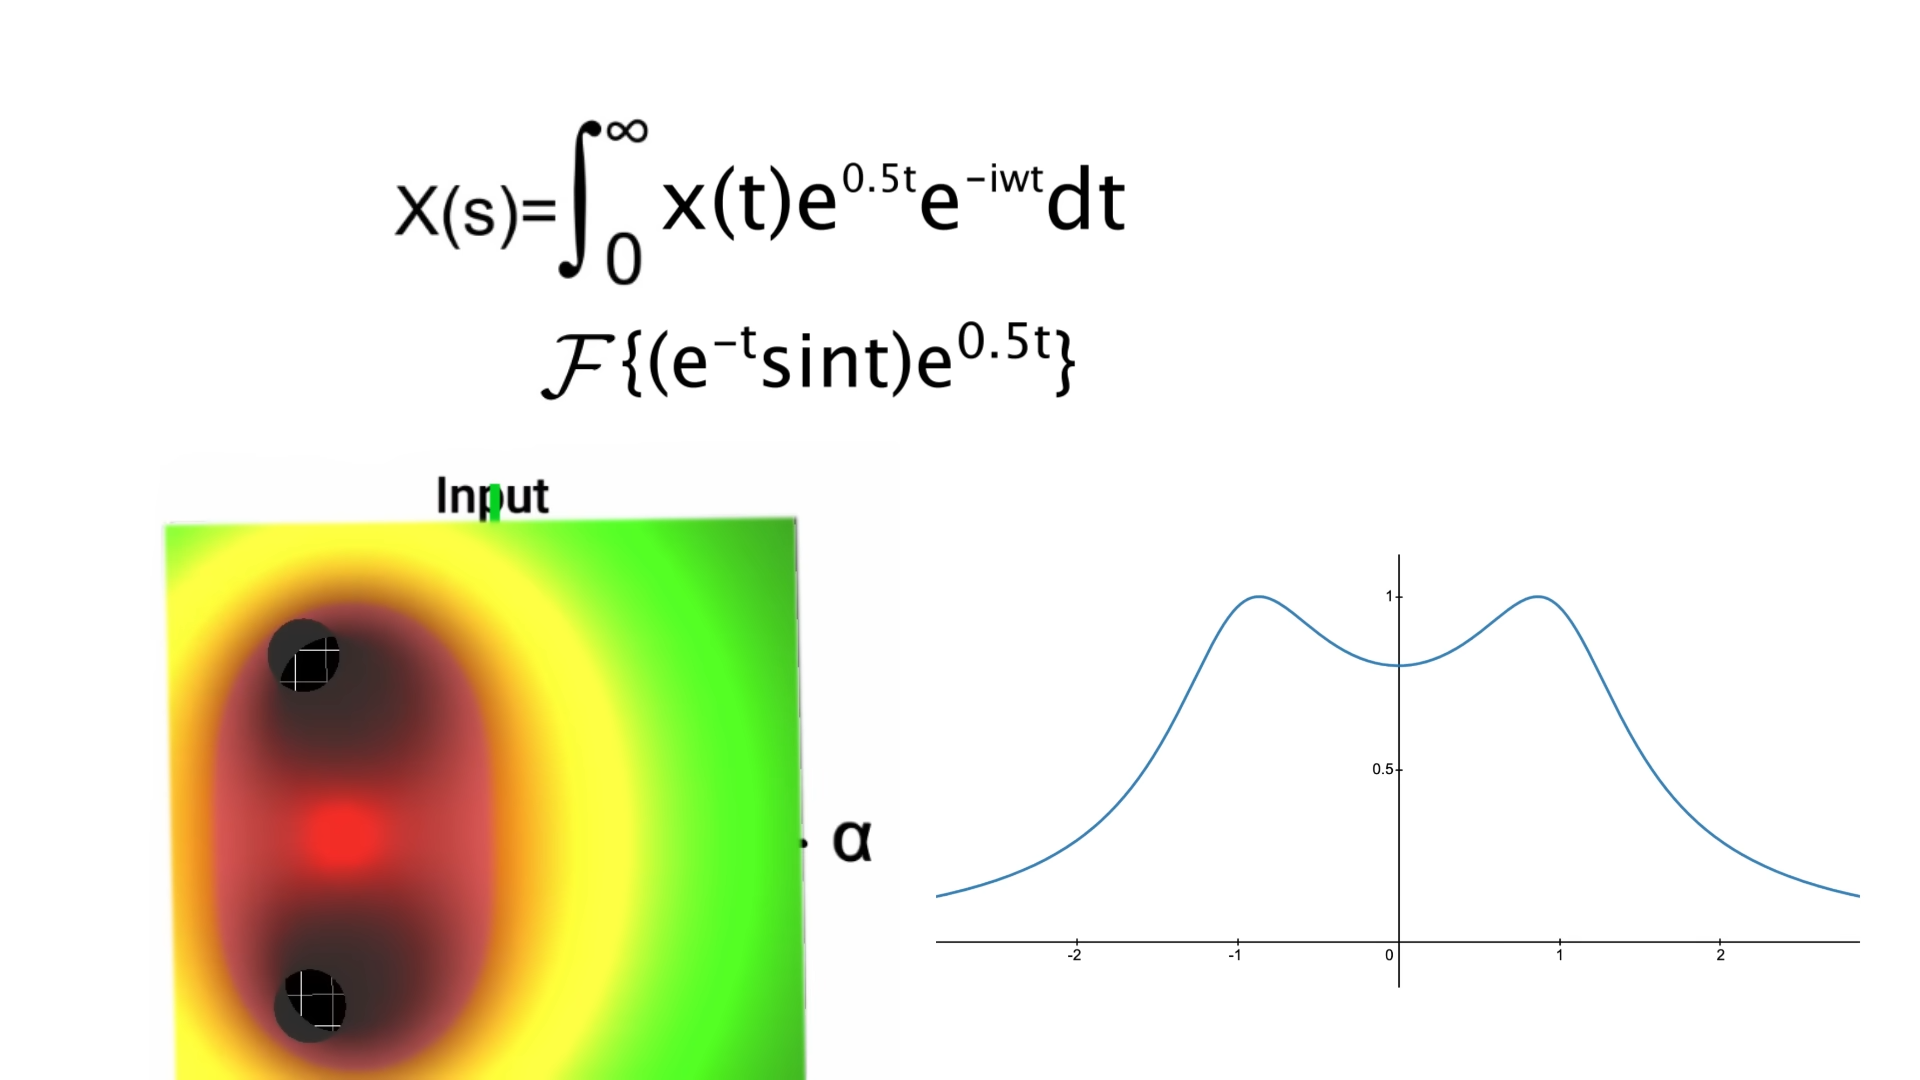
\includegraphics[width=1\linewidth]{Laplace_03_graph.png}
    \end{figure}
    See the animation for the complete visualization: \url{https://youtube.com/clip/UgkxEzdqZqm4uYFIgYPmoLHf6dGBKRtj7TXh?si=VI5mkUaOHnu5nGqc}
\end{frame}

\begin{frame}{Laplace Transform}
        The imaginary coordinate is $1$ and $-1$, which matches the coefficient or angular frequency of our sinusoid, $\sin t$. The real component $-1$ matches the coefficient in the exponential term, $e^{-t}$.\\
        Here is the full animation: \url{https://youtube.com/clip/UgkxCi_tdc5WwrOrwwwkra50Si3TYPwJgIxn?si=sUwSRDF242P1nY-K}
\end{frame}

\end{document}